%!TEX root = ../BGP_for_networks_who_peer.tex
\chapter{Becoming multi-homed}
\section{What is being multi-homed (in terms of BGP)?}
In the last chapter, we set up eBGP to one ``upstream'' provider. But in practice, this is not what we want - we would be dependent on only one connection to the outside world and would be offline if it failed (which is exactly the same as running no BGP at all).

So we need to connect to (at least) one more upstream. And to make our network even more resilient and to drive down cost, we will also connect to an Internet Exchange and set up peering sessions there.

This increases our network (and BGP) complexity somewhat, but if we plan (and configure) carefully, then this complexity is easily manageable. The purpose of this chapter is to offer you best practices, so that you do not run into an over-complex network set-up later on.

\section{What changes when you become multi-homed?}
When you have only one connection to the outside, your world is simple:
\begin{itemize}
  \item You either have a default route to your upstream and send everything which is not inside your own network to there, or
  \item you get a full routing table from your upstream, but still have only one connection to the outside to send traffic to.
\end{itemize}

With two (or more) connections to the outside, it gets more interesting:
\begin{itemize}
  \item You receive the same prefix(es) via BGP from provider A and provider B; which one do you prefer?
  \item What criteria does BGP use per default to decide which prefix announcement is ``better''?
  \item Can you influence or override this decision? (yes, you can)
  \item When to influence best prefix selection (this is what this is called) and when to leave it to the defaults? (this is lifelong learning).
\end{itemize}

\section{Configuring multi-homing}
\subsection{Network setup}
\begin{figure}
  \centering
  \includegraphics[width=\linewidth,page=3]{img/Drawings.pdf}
  \caption{Example setup with two upstream providers and peering}
  \label{fig:multihoming}
\end{figure}
See figure \ref{fig:multihoming} for our example network. Your AS64500 is connected two upstreams AS64496 and AS65550. Behind them we have a couple of ASes for distributing prefixes - their AS numbers are not really important. One of them also peers with you.

\subsection{Receiving prefixes}
For our somewhat simplified view of the Internet, we receive a handful of prefixes originated by AS517 over various paths.
\iffalse
Configure your router according to the experiment sheet and have a look at your BGP table to see which prefixes are considered ``best''.
\fi

\subsection{Sending prefixes}
You should always only send your own prefixes and those of your customers. Beware - if you do not configure any filtering, your router sends out \emph{all best prefixes} it knows about. So if you connect to two upstream providers, you announce  your full routing table to both of them unless you implement some filtering.

\section{Configuration examples}
These examples are purposely IPv4, merely to make them easier to read. Adding IPv6 is done according to the same principles as shown in chapter \ref{ch:eBGP}.

\subsection{Cisco example}
\begin{verbatim}
  router bgp 64500
    neighbor upstream peer-group
    neighbor upstream route-map upstream-in in
    neighbor upstream route-map upstream-out out
    neighbor upstream route-map send-community both
    neighbor upstream route-map soft-reconfiguration inbound
    !
    neighbor 10.200.2.1 remote-as 64496
    neighbor 10.200.2.1 peer-group upstream
    !
    neighbor 10.230.2.1 remote-as 65550
    neighbor 10.230.2.1 peer-group upstream
    !
    neighbor peering peer-group
    neighbor peering route-map peering-in in
    neighbor peering route-map peering-out out
    neighbor peering route-map send-community both
    neighbor peering route-map soft-reconfiguration inbound
    !
    neighbor 80.81.193.66 remote-as 286
    neighbor 80.81.193.66 peer-group peering
\end{verbatim}
You see that we reference four route-maps here. For the moment we will just keep them  empty; later we will add statements to them:
\begin{verbatim}
  route-map upstream-in permit 100
  route-map upstream-out deny 100
  route-map peering-in permit 100
  route-map peering-out deny 100
\end{verbatim}
The incoming route-maps permit everything, the outgoing route-maps deny everything.

\subsection{Mikrotik example}
Mikrotik does not support peer groups, every peer entry needs every parameter.
\begin{verbatim}
  /routing bgp instance
  set default as=64500 out-filter=bgp-out router-id=\
    192.168.1.1

  add in-filter=upstream-in name=AS64496 out-filter=upstream-out \
      remote-address=10.200.2.1 remote-as=64496
  add in-filter=upstream-in name=AS65550 out-filter=upstream-out \
      remote-address=10.230.2.1 remote-as=65550

  add in-filter=peering-in name=AS286 out-filter=peering-out \
          remote-address=80.81.193.66 remote-as=286
\end{verbatim}
We also have defined filter lists here; for the moment, we will keep them empty:
\begin{verbatim}
  /routing filter
  add chain=upstream-in action=accept
  add chain=upstream-out action=reject
  add chain=peering-in action=accept
  add chain=peering-out action=reject
\end{verbatim}

\subsection{FRRouting example}
(the same as for Cisco IOS)
